\documentclass{article}
\usepackage[utf8]{inputenc}
\usepackage{amssymb}
\usepackage{tikz}
\usepackage{amsmath}
\usepackage{relsize}
\usepackage{mathtools}
\usepackage{textcomp}
\usepackage{eurosym}
\usepackage{amssymb}
\usepackage{systeme}
\usepackage{mathtools}
\usepackage{graphicx}
\usepackage{subfig}
\usepackage[bottom]{footmisc}
\usepackage{mwe}
\usepackage{csquotes}
\usepackage[colorinlistoftodos]{todonotes}
\usepackage{subfig}
\usepackage{color,soul}

\title{Method}
\author{Roman Oort}
\date{\today}

%%% PERSONAL SHORTCUTS
\DeclareMathOperator*{\plim}{plim}
\newcommand{\T}{\textbf{T}}
\newcommand{\Tij}{\textbf{T}_{ij}}
\newcommand{\Soc}{(\T(n))^{\infty}_{n=1}}
\newcommand{\beli}[3][2]{p_{#2}^{(#3)}}
\newcommand{\belvec}[2]{\textbf{p}^{(#2)}}

\begin{document}

\maketitle

\tableofcontents
\newpage

\section{Network Generation}

\subsection{Random Generation}
\label{generation:random}
In order to allow for proper analysis of the DeGroot mechanics a method to generate \emph{random} networks was created, to ensure generality of the obtained results. Given a number of agents this method is capable of generating both directed and undirected networks, and accepts several other parameters to shape the generation as desired.

\subsubsection{Default Case}
In the default, most basic, case this function simply takes the desired number of agents, $n$ as input. Other, optional, parameters can be provided to customize the desired network and will be discussed in detail at the relevant time.
To start, an empty $n\times n$ array \cite{2020NumPy-Array}, i.e. containing solely zeroes, is created, which serves as a blank slate for the interaction matrix $\T$ of the network\hl{, which is all that is required to describe a network as discussed in [REF].}\todo{Possibly unnecessary}
Subsequently the function will iteratively add the links for every agent in the network, in order to ensure the generated network is fully connected at every size. \newline
In this iteration there is one special case, namely, the very first agent. To ensure aperiodicity, as discussed in [REF], and therefore convergence, the very first agent is guaranteed to receive a self-link. As this creates a cycle of length one, aperiodicity is guaranteed. \newline

Every subsequent agent, when generating a directed network, will be guaranteed to both receive and send one link. When generating an undirected network each agent is guaranteed to have one link, which is both incoming and outgoing. This guarantees that the network of size $n$ will be fully connected. However, as the interest lies in sequences of networks, all of which need to be convergent, this condition needs to be met by every network in the sequence of size $n^{\prime} < n$, not only by the network of size $n$. Therefore, these guaranteed links will be sent to, and by, an earlier agent in the network, that is to say that the guaranteed links of an agent $k$ can only be sent to and received by any agent $m < k$. This guarantees the strong connectedness of the network, at every size, which can be proven inductively [REF]. This also holds for an undirected network, where the only difference is that the agents receiving and sending a link are one and the same. The specific agents on the other end of these guaranteed links are sampled randomly from a uniform distribution over the interval of agents already present in the network. \newline

Therefore, as this method of generation not only guarantees connectedness in the total network, but also at every smaller size of the network, this returned network can also be considered a sequence of networks. To access a network of a specific size in this sequence, one would only need to take the rows and columns up to that size to obtain the specific network. This ensures that the network and its links stay constant between sizes, allowing for proper comparison of different networks in the sequence. Finally, this function is also capable of growing an existing network: when a matrix and a positive integer $m$ are provided, the function will grow this existing matrix by adding $m$ rows and columns, one for each agent, whose links are determined in the same way as described earlier.\newline

This method of generating these network was chosen over more standard methods of model generation for several reasons. For starters, implementing the network generation from scratch provides more low-level control over the network generation process, allowing more options for customization. A clear effect is the strong connectedness mentioned earlier. Using another method for generating the network, while possibly faster when initially generating the network, would require another pass over all agents to ensure the network is fully connected, and remains so at every size. 

Another, more subtle, effect of the chosen method is a slight bias towards the earlier agents in the network, an effect which can be seen in figure (\ref{degree:agent}) below, which shows the average degree for each consecutive 100 agents. As shown earlier the agents are added to the network the higher their degree tends to be. This mirrors how those individuals who are part of a group for a long time tend to have more connection than those new to the group.

\begin{center}
    \begin{figure}[!htbp]
        \centering
        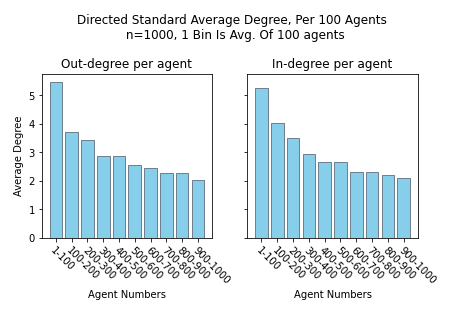
\includegraphics[width=.8\textwidth]{ThesisKI/Images/DirectedStandardPerAgent.png}
        \caption{Average Degree per 100 agents}
        \label{degree:agent}
    \end{figure}
\end{center}
\newpage
\subsubsection{Customization}

As mentioned the chosen implementation has the option to adjust the generation process as desired. These adjustment are applied complementary to the default generation, to ensure the base guarantees of this method. \newline

First of all, this method allows for the generation of both directed and undirected networks. The method for generating undirected networks is very similar to the generation of directed networks. In fact, the process is entirely the same, save for one detail. In contrast to the generation of a directed network, where the agents to receive and send a link are chosen independently, and therefore tend to be distinct agents, the generation of an undirected network simply chooses one random agent to both receive and send a link. After all, the only difference between the interaction matrix $\T$ of a directed and undirected network is that the matrix of an undirected is symmetrical, whereas the matrix of an undirected network is asymmetrical. \newline
Furthermore, when a directed network is created it can be made into an undirected network. This is done by simply taking the element wise maximum between the original matrix and its transpose, effectively mirroring all links in the matrix along the diagonal. \newline

Secondly, there is also the option to increase the degree of the agents to more than the base minimum. Using the default generation results in nearly half of all agents having only two links, the bare minimum \footnote{In a network where every agent is guaranteed a self-link}, with a quickly dissipating tail on this distribution as demonstrated in figure (\ref{deg:std}). However, when using this option to increase the degree of the network, this distribution is spread out more evenly and is flattened, leading to a more even distribution of degrees, as seen in figure (\ref{deg:inc})
\begin{figure}[!htbp]
  \centering
  \subfloat[Standard Degree]{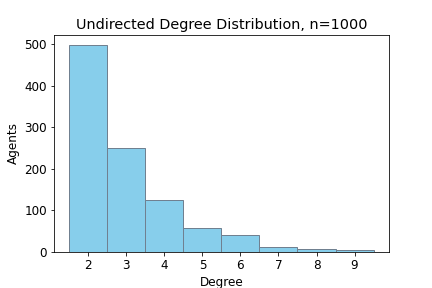
\includegraphics[width=0.5\textwidth]{ThesisKI/Images/DegreeUndirectedStd.png}\label{deg:std}}
  \hfill
  \subfloat[Increased Degree]{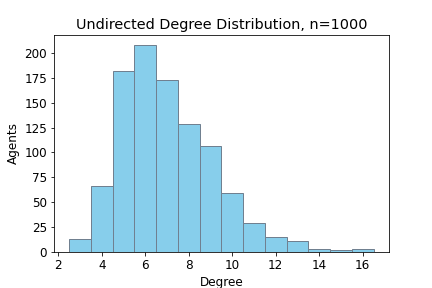
\includegraphics[width=0.5\textwidth]{ThesisKI/Images/DegreeUndirectedInc.png}\label{deg:inc}}
  \caption{Degree Distributions Undirected Network}
\end{figure}

\newpage

The procedure for increasing the degree of a network occurs during the generation procedure. During the iteration, each agent samples a random number to increase their degree by, sampled from a given distribution, by default $\mathcal{N}(2,1)$, which was also used to generate figure (\ref{deg:inc}). This number is then rounded to the nearest integer, and, when this integer is positive, the agent will receive this amount of additional links. Once again the agents on the other end of the link are sampled randomly from a uniform distribution, this time over \emph{all} agents, not only over those already present in the network, and the corresponding element in the matrix is then set to one. When this method is used for an undirected network only one number is drawn to increase the degree, however, for a directed network two number are sampled, for both the in-degree and the out-degree.
The probability distribution, and its respective parameters, from which the degree increase is sampled can be changed to influence the distribution of degree as much as desired.
\newline

A final option for the customization of the network generation is the probability of a self-link, which can be set at the moment of generation. This sets the probability for each agent to form a link with itself, save for the first agent, which always receives a self-link in order to ensure the aperiodicity of the network.
\begin{center}\todo{increase font-size}
    \begin{figure}[!htbp]
        \centering
        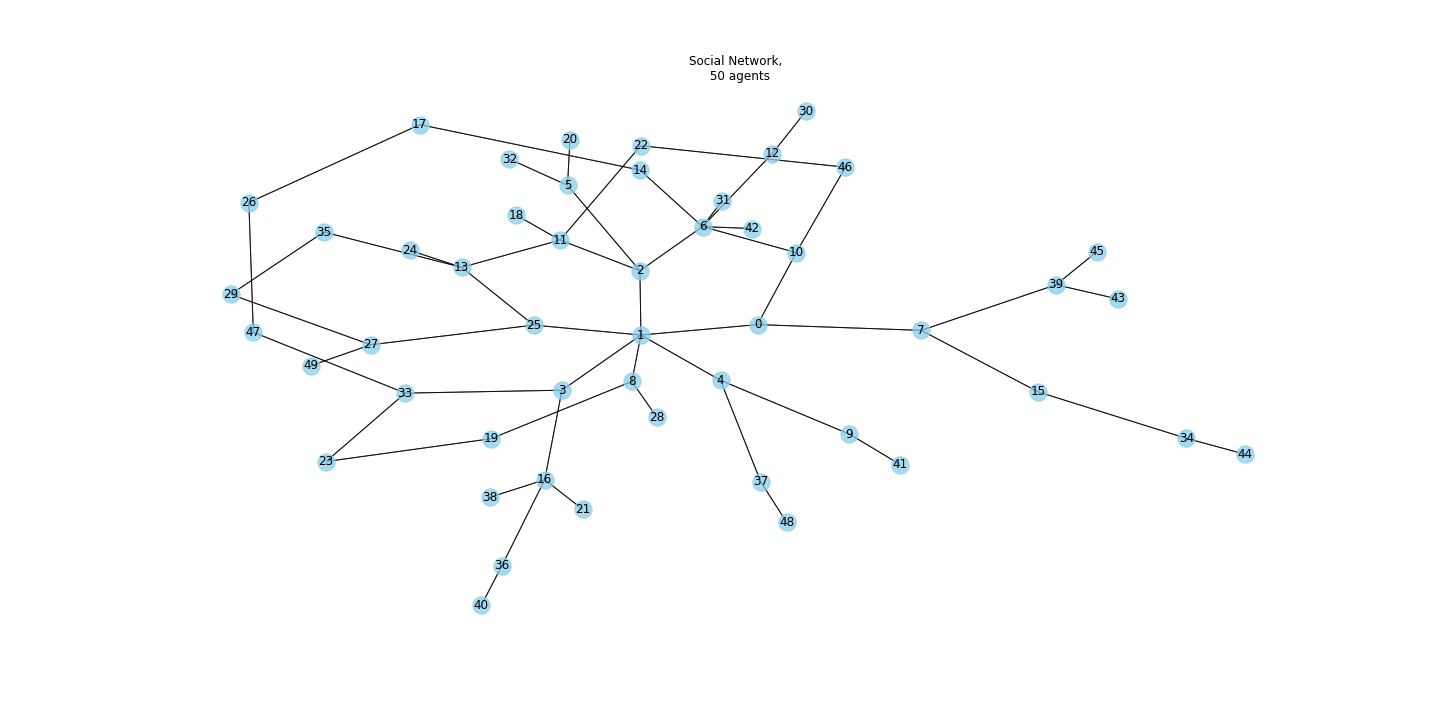
\includegraphics[width=1.1\textwidth]{ThesisKI/Images/NoneGraphRandom.png}
        \caption{Example of Randomly Generated Undirected Network}
        \label{network:random}
    \end{figure}
\end{center}

\newpage

\subsubsection{Sparse Matrices}

One caveat of the chosen implementation is the memory consumption. As the interaction matrix is two-dimensional its size increases in a polynomial manner. As the wisdom of crowds effects occurs as the network size approaches infinity this poses a problem, with large networks consuming a large amount of memory. In order to circumvent this problem the implementation of the network generation stores the interaction matrix in a sparse format \cite{2020SciPy-NMeth}. As can be seen in figure (\ref{generation:memory}) this decreases the memory consumption to negligible levels, for networks of up to $10,000$ agents, whereas when using a standard, dense, matrix the memory consumption increases rapidly. \newline
However, generating a network as a sparse matrix is a somewhat slower process than generating the same network as a dense matrix, though both generation processes still run in linear time as can be seen in figures (\ref{generation:time_inc} \& \ref{generation:time_std}),  which show the network generation times for a network with increased degree, and standard degree respectively. Therefore, as the generation of the network needs only be run once, the decrease in memory usage was considered to outweigh the slightly increased run-time, and the sparse generation was chosen as default.

\begin{figure}[!htbp]
    \centering
    \subfloat[]{\label{generation:memory}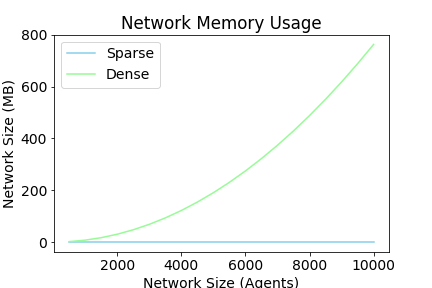
\includegraphics[scale=.45]{ThesisKI/Images/Memory.png}}
    
    \begin{minipage}{.5\linewidth}
    \centering
    \subfloat[]{\label{generation:time_inc}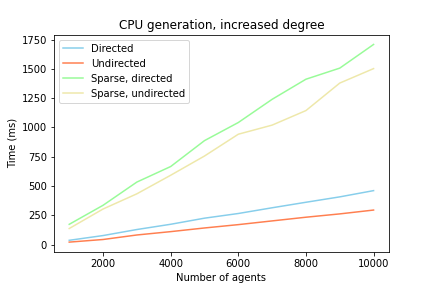
\includegraphics[scale=.4]{ThesisKI/Images/CPU_inc.png}}
    \end{minipage}%
    \begin{minipage}{.5\linewidth}
    \centering
    \subfloat[]{\label{generation:time_std}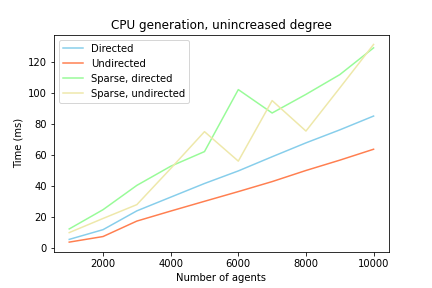
\includegraphics[scale=.4]{ThesisKI/Images/CPU.png}}
    \end{minipage}\par\medskip
    \caption{Network generation, \\ memory and time consumption}
\end{figure}


\section{Belief Initialization}

The generation of the beliefs follows the procedure as discussed in section [REF]. That is to say, the initial opinion of an agent $i$, $\beli{i}{0}$, is generated by adding a random, independently sampled, zero-mean, error term, $e_i$, to the assumed truth of the network. This is implemented by generating an array of length $n$, where each entry is sampled from a zero mean probability distribution, $\mathcal{N}(0, 0.75)$ by default. The assumed truth, $\mu$, is drawn randomly from a uniform distribution on the interval $[0, 1]$, and is added to each entry in this array of error terms. \newline
However, as mentioned in section [REF] all beliefs are to lie on the interval $[0, 1]$, which is not guaranteed with this method. After all, as $\mu$ is chosen randomly it can lie arbitrarily close to the edges of the interval, allowing for the a very small error term to push the belief outside of the interval. What's more, the probability distribution is continuous, meaning it is even possible for an error term to be larger than $1$.  Therefore, in order to force each belief onto this interval the initial belief vector is value normalized, according to following rule:
\begin{equation*}
    \beli{i, \text{norm}}{0} = \frac{\beli{i}{0} - \min(\textbf{p}^{(0)})}{\max(\textbf{p}^{(0)}) - \min(\textbf{p}^{(0)})},
\end{equation*}
which ensure that the smallest belief in the belief vector is normalized to $0$, the highest belief normalized to $1$, and every other belief will fall somewhere in between. However, as this shift the mean of the belief vector away from $\mu$, $\mu$ itself must undergo the same normalization in order to ensure each belief is still properly generated from this value.
\newline

\section{Weight Initialization}

The previous method does instantiate the network, by creating the links between all agents. However, it does not yet place a weight on all of these links, to describe how much weight agents place on the beliefs of others. For this purpose different options to initialize the weights have been determined. These are all applied only on the non-zero entries in the interaction matrix, therefore they do not create any new links, nor do they remove those already existing links, potentially disrupting the connectedness of the network.

\subsection{Uniform}

The first, default, weight initialization is uniform weighting. This simply means that every agent places the exact same weight on the opinions of every other they are connected to. The implementation amounts to simply let the interaction matrix $\T$ remain as is, with a $1$ indicating a link and a $0$ indicating no link.

\subsection{Overlap}

The second initialization is based on the idea that an agent prefers to receive information from as many different sources as possible. The weight placed on an agent is therefore proportional to the amount of new information they are able to provide, based on the overlap in neighbours between two agents, where agents' neighbours are those other agents with whom they have a link. The weight initialization is based on the following rule:
\begin{equation}
    \T_{ij}(n) = 1 - \alpha \cdot \frac{|N_i(n) \cap N_j(n)|}{|N_i(n)|},
\end{equation}
which essentially subtracts the fraction of overlap between the set of neighbours of agents $i$ and $j$ from the weight that $i$ places on $j$. This fraction is then multiplied with a discount factor $\alpha \in [0, 1)$ to ensure that a link between agents is not deleted in the event that their neighbouring sets perfectly overlap. 

\subsection{Belief}

Another method of setting the weights between agents is based on the idea that agents are more willing to pay attention to those around them with the same mindset. The weight that one agent places on another is based on their difference in opinion: the more similar their opinions the more weight they attribute to the other's opinion, and vice versa. First, in order to set the weights this way, the initial belief vector is concatenated with itself $n$ times, to form an $n \times n$ matrix where each column is the belief vector at $t=0$, as follows:
\begin{equation}
    B(n) = [\textbf{p}^{(0)}(n)]^{n}
\end{equation}

In order to get the difference in belief between any two agents, the transpose of the matrix formed by concatenating the belief vectors can simply be subtracted from the matrix itself. Then, for every non-zero element in $\T$, the weight is set as the absolute difference in opinion subtracted from 1, as follows:
\begin{equation}
    \T_{ij}(n) = 1 - \alpha \cdot |B_{ij}(n) - (B^{T})_{ij}(n)|
\end{equation}

Again, just as in the overlap initialization, $\alpha$ is a discount factor on the interval $[0, 1)$ to prevent deletion of links, should two connected agents hold perfectly opposed beliefs.

\subsection{Random}

Another method of initializing the weights of the network is to simply generate the the weights randomly. This method generates an $n \times n$ matrix filled with numbers sampled from a given distribution, and corresponding parameters, a uniform distribution on $[0, 1]$ by default. In order to ensure the weights are applied only to existing links the randomly generated matrix and the interaction matrix $\T$ are multiplied element-wise, as each element of the $\T$ matrix at this point is either $1$ or $0$.

\subsection{Self-links}

One final hiccup in the weight initialization are the self-links. When using either uniform or random weights everything works as intended. However, when setting the weight based on either overlap of belief unintended behaviour occurs. Namely, when setting the weights based on overlap, a self-link will always be assigned the lowest possible weight. After all, two identical sets, in this case the overlap between the sets of neighbours of agents $i$ and $i$, will perfectly overlap.
Conversely, when setting the weights based on beliefs, a self-link will always receive the highest possible weight. After all, the difference in opinion between an agent and themselves will always be $0$. \newline
In order to circumvent this, when initializing the weights using one of the aforementioned methods, the self-links will be assigned a random weight, sampled from a normal distribution whose mean and standard deviation are taken to be the mean and standard deviation of all other weights in the network. This ensures that the self-links are generated to be more in line with all other weights in the network.

\subsection{Normalization}

Finally, in order to achieve convergence, it is necessary that $\T$ is row-stochastic, meaning its elements sum to one, row-wise. In order to ensure this condition, after the weights have been initialized, the matrix is normalized row-wise as follows:
\begin{equation}
    \T_{ij, norm}(n) = \frac{\T_{ij}(n)}{\sum_{j}\T_{ij}(n)}
\end{equation}

In other words, each entry is simply divided by the sum of all weights in the corresponding rows. While this does not preserve the exact values given to the weights by the initialization function, it does preserve their values in relation to the other weights in the row, which is the most important.

\newpage

\section{Non-cooperative Agents}

Now, having the ability to generate a cooperative network of a given size, what remains is the ability to add non-cooperative agents without disrupting the benefits obtained by the chosen method of network generation.
Furthermore the implementation has to have the ability to switch a network between cooperative and non-cooperative at will, to allow for proper comparison between those networks.
Therefore the generation of the non-cooperative agents occurs after the cooperative part of the network has already been generated. Iterating over the given number of non-cooperative agents, each of them receives a random selection of agents with whom they will have a link, the number of which will be equal to the average degree of the network, at its full size.
In addition to the randomly selected agents each non-cooperative agent is guaranteed to receive a link to one of the first five agents in the network. This is done to make sure that the non-cooperative agents will still have links to others, even when the observed network is relatively small.

The links of these non-cooperative agents are then stored to allow them to be added to a network of any size. In order to add them to any network in the sequence, regardless of size, first empty rows are concatenated to the interaction matrix. After all, what distinguishes non-cooperative agents from their cooperative counterparts is their lack of incoming links, which is expressed by empty rows in the interaction matrix. After the empty rows are added, the respective columns are added, representing those agents who listen to non-cooperative agents. The regular interaction matrix of size $n \times n$ is therefore extended to a matrix of size $n+m \times n+m$, where $m$ is the number of non-cooperative agents.
An example of a resulting non-cooperative network can be seen in figure (), below, where the non-cooperative agents are labeled in red.

\section{Updating Rules \& Convergence}

In order to compare the different variations on the DeGroot mechanics these variations all needed their respective updating rules to be implemented.

\subsection{DeGroot}

As shown in section [REF]\todo{ref naar updating rule section} $\textbf{p}^{(t)}$ can be computed two different ways. The first is the iterative method described in equation [REF] \todo{ref naar iterative updating method}, simply multiplying the belief vector at the previous time-step, $\textbf{p}^{(t-1)}$, with the interaction matrix, $\T$, and repeating this process $t$ times. In order to converge a network, using the standard DeGroot dynamics, this process is repeated, until the difference between $\textbf{p}^{(t)}$ and $\textbf{p}^{(t-1)}$ is zero, or near enough. In other words, the updating step is applied until the beliefs no longer change from one step to another.

The second is to use the method described in equation [REF] \todo{ref naar verkorte updating rule}, which states that to compute the belief vector for a specific $t$, the initial belief vector can be multiplied with the interaction matrix, raised to the power of that $t$. However, upon examination of the computational time, as shown in figure \ref{update:time}, [REF] \todo{ref naar exponentiation update rule}, is significantly slower, for both dense and sparse matrices.
\todo{fontsize}
\begin{figure}[!htbp]%
    \centering
    \subfloat[\centering Dense Matrix]{{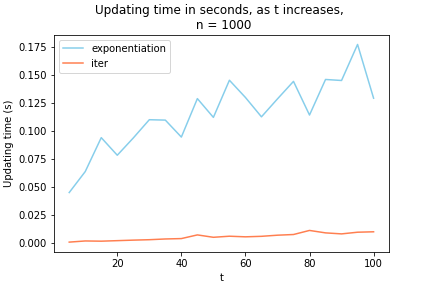
\includegraphics[width=.45\textwidth]{ThesisKI/Images/UpdatingTimeDense.png} }}%
    \qquad
    \subfloat[\centering Sparse Matrix]{{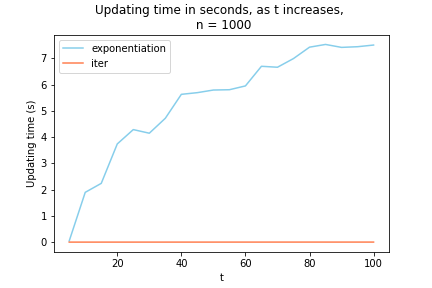
\includegraphics[width=.45\textwidth]{ThesisKI/Images/UpdatingTimeSparse.png} }}%
    \caption{Updating time}%
    \label{update:time}%
\end{figure}

Therefore the iterative method was implemented, in order to significantly speed the updating process. Furthermore, this also allows for saving all intermediate belief vectors, providing insight in the rate of convergence of the network.

However, as shown by \cite{degroot1974concensus}, the convergent belief can also be computed directly, using the eigenvector of the interaction matrix, $\T$, corresponding to $\lambda=1$. Therefore another function was made for those cases where only the convergent belief is of interest. This function gives only the convergent opinion of the network.

\subsection{$\varepsilon$-DeGroot}
\subsubsection{Standard}

The second updating rule that can be sued to converge a network is the $\varepsilon$-DeGroot variation mentioned in section [REF]\todo{ref naar section $\varepsilon$}. The general framework is the same as for standard DeGroot method: repeatedly apply the updating rule until the beliefs stop changing. However, to converge a network using this method a slight modification is necessary. First of all under the $\varepsilon$-DeGroot dynamics the belief vectors do not adhere to the standard notion of convergence as under regular DeGroot dynamics, rather, using this updating rule results in what \cite{amir2021robust} describe as \textit{alternating convergence}. That is to say, rather than one single convergent belief vector, there are two convergent belief vectors, between which the agents alternate.
Therefore, using the same condition for convergence as regular DeGroot mechanics will result in an infinite loop, as the belief vectors will alternate, ensuring there will always be a difference between the beliefs at $t$ and $t-1$. To this end, the convergence condition is changed somewhat. Rather than comparing the beliefs between $t$ and $t-1$ only, the belief vectors are compared between $t$ and $t-2$, to check whether their difference is 0, or near enough. This is also done for the beliefs at $t-1$ and $t-3$ to check whether both of the alternating belief vector have converged. As long as convergence has not occurred for both belief vectors the agents the process keeps repeating.

\subsubsection{Alternative}

The alternate $\varepsilon$-DeGroot dynamics work similarly to the standard $\varepsilon$-DeGroot updating rule, as described in [REF] \todo{ref naar alt $\varepsilon$}. Similarly, it also displays \textit{alternating} convergence, rather than the more standard notion of converge. Therefore, in order to properly detect when the network has converged the same conditions for converge are used as with the standard $\varepsilon$-DeGroot mechanics.

\subsection{Private Belief}

Another updating rule implemented allowed each individual agent to account for a private, constant, belief when updating their opinion. In the chosen implementation this private belief was chosen to be the initial belief at time $t=0$. This way agents will always place some amount of weight on their initial belief. The weight placed on this initial belief is specified by the parameter $\alpha \in [0, 1]$. Converging a network using this updating rule, follows the same process as regular DeGroot mechanics, i.e. repeatedly applying the updating rule until the belief vector no longer changes between iterations. As this updating method results in the more standard notion of convergence, opposed to \textit{alternating} convergence, no further modifications to the convergence procedure were required.

\subsection{Threshold}

Another, minor, modification to the regular DeGroot updating mechanics imposes a threshold on the updating rule, ensuring that agents do not drastically change their opinion in a single updating step. Whenever an agent changes their opinion between two time-steps they can change their opinion by no more than the given threshold, effectively limiting how volatile an agents opinion is, simulating a hesitancy in rapid, drastic, changes in opinion.

\subsection{Variable Weights}

\newpage
\section{Appendix}
\subsection{Proof of (strong) connectedness}

\textbf{Base Case:} \newline
Let $S_1$ be a random social network of 1 agent, generated using the method described in \ref{generation:random}.
S is guaranteed to be fully connected, as the first agent in a network always receives a self-link.\newline

\textbf{Induction Hypothesis:}\newline
Let $S_n$ be an arbitrary, strongly connected, randomly generated network, obtained by the method described in \ref{generation:random}. Now let $S_{n+1}$ be the network that is obtained by growing the network $S_n$ by one agent. We now want to prove that if $S_{n+1}$ is grown from $S_n$ using the method from \ref{generation:random}, $S_{n+1}$ is also strongly connected.\newline

To grow the network $S_n$ by one agent, the agent $n+1$ is added to the network, with two guaranteed links, one incoming and one outgoing. Let the $i$ and $j$ be the arbitrary agents involved in these links, respectively. By the generation procedure outlined in \ref{generation:random}, these agents are guaranteed to be present in $S_n$. However, by our induction hypothesis we now that $S_n$ is strongly connected, therefore there exists a directed path from $i$ and $j$ to any other agent in the network. Therefore, as agent $n+1$ has an incoming link from agent $i$, there exists an incoming path from any agent in the network to $n+1$, and, furthermore, as $n+1$ has an outgoing link to agent $j$, there also exists an outgoing path to any agent in the network. Therefore, as there exists a directed path to any agent in the network from agent $n+1$, $S_{n+1}$ must be strongly connected.\newline
Therefore, as $S_n$ and $S_{n+1}$ were arbitrary networks, it must be the case that any network generated using this method must be strongly connected.\newline

\bibliographystyle{apalike}
\bibliography{references.bib}

\newpage
\end{document}